\section*{Speed of light}

\begin{equation}
T_1 = \frac{X+}{den}
\end{equation}


\begin{figure}[h!]
\centering
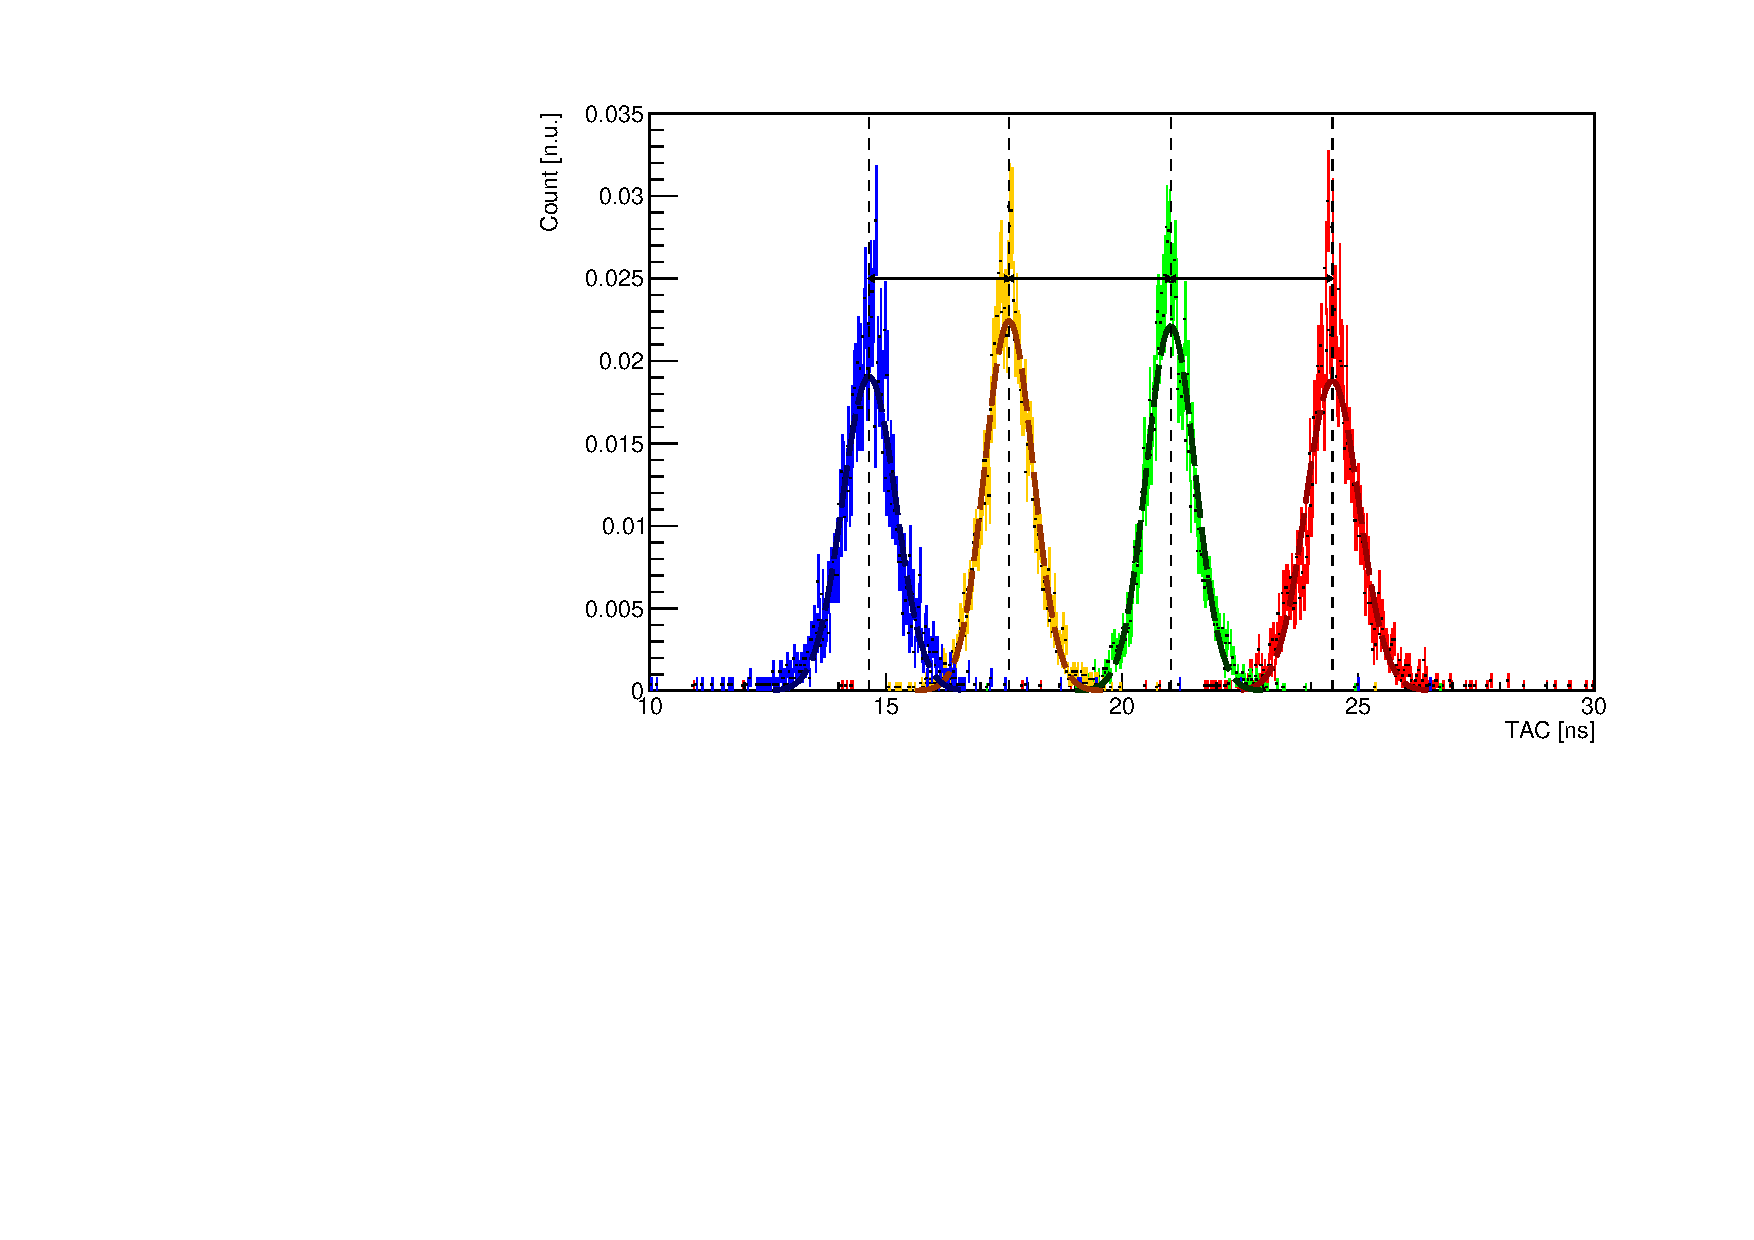
\includegraphics[width=0.8\textwidth]{TACoverlayed_dist}
\caption{TAC distribution in the four different positions.}
\end{figure}
 
\begin{figure}[h!]
\centering
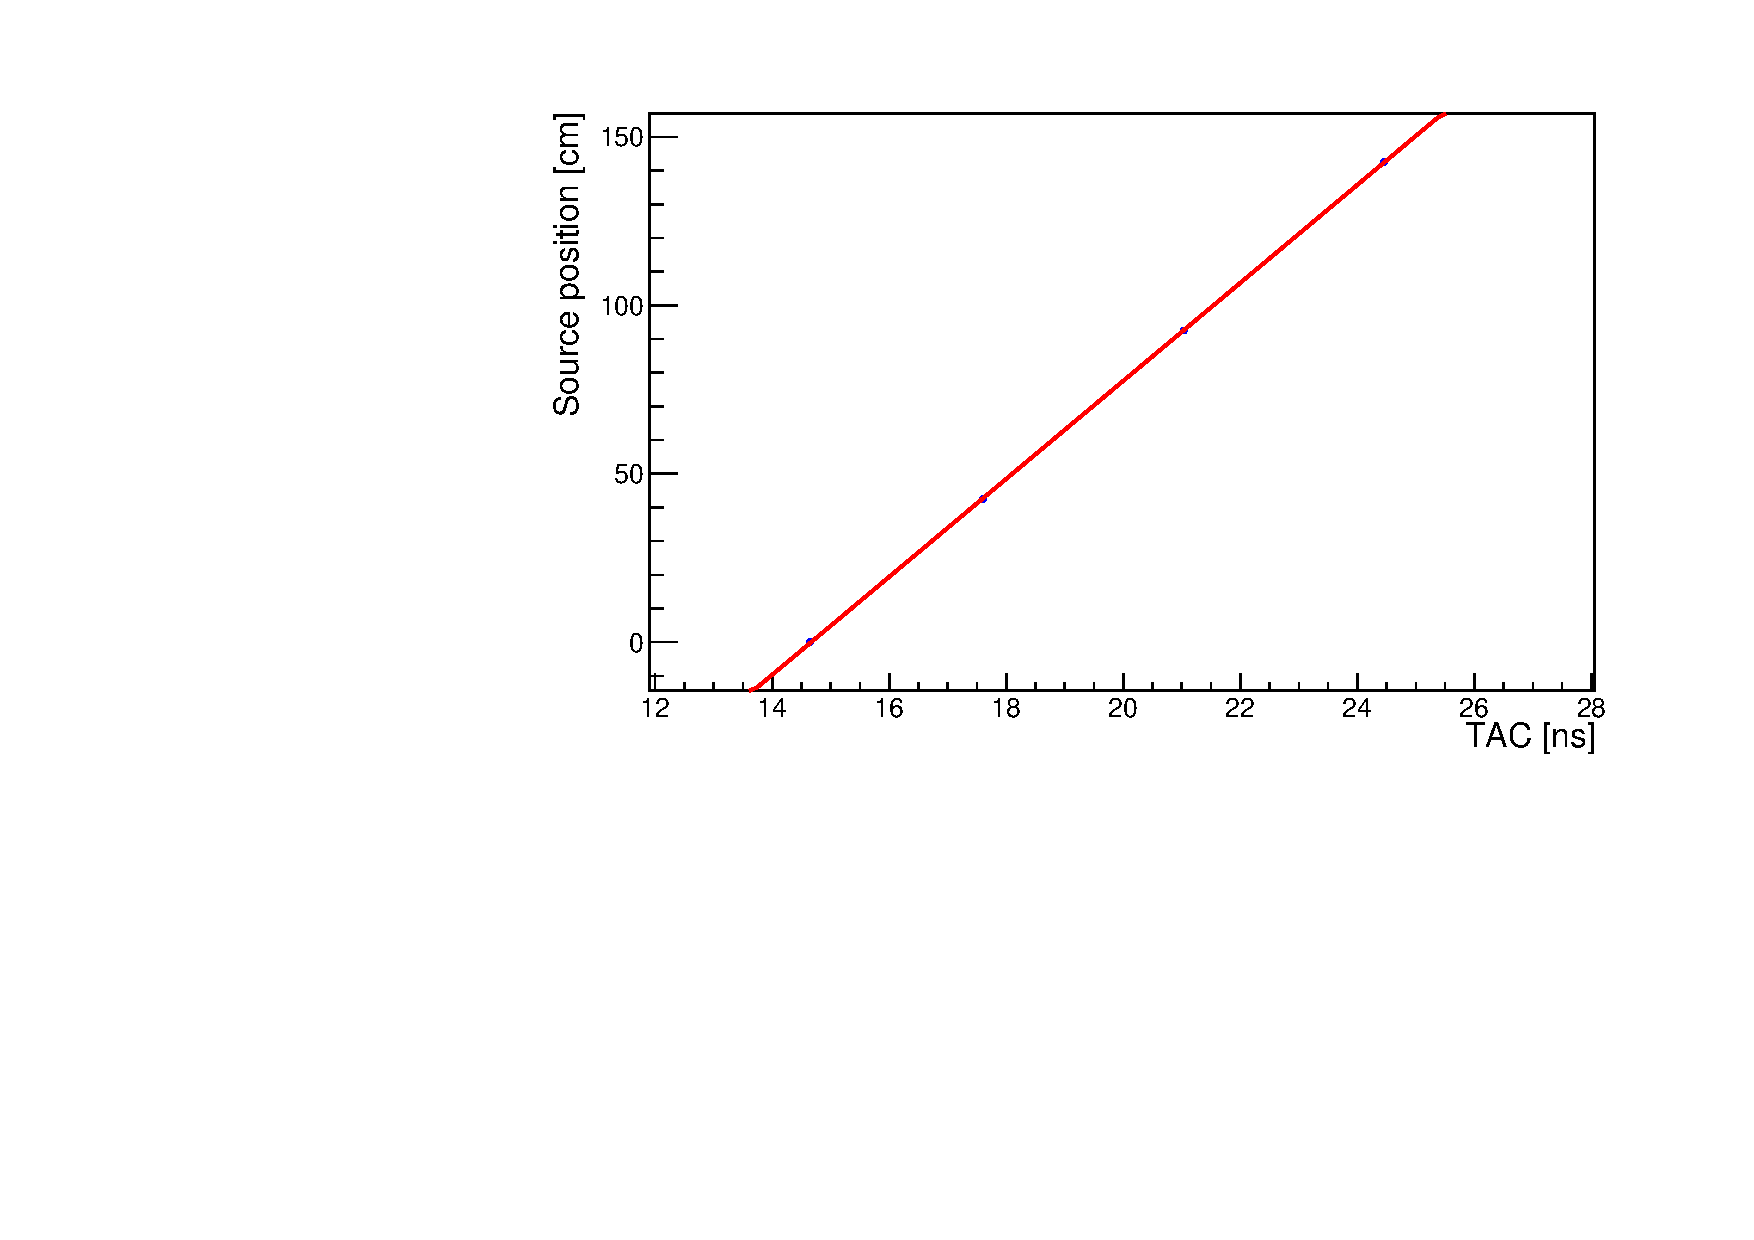
\includegraphics[width=0.8\textwidth]{Speed_fit}
\caption{Position vs Time (the angular coefficient is c/2).}
\end{figure}
